\documentclass[c,unicode,russian]{beamer}
\usepackage{hyperref}
\usepackage{alltt}
\usepackage{verbatim}
\usepackage{fancyvrb}

\usepackage{fontspec}
\setsansfont{Ubuntu}
\setmonofont{Ubuntu Mono}
\usepackage{polyglossia}
\setdefaultlanguage{russian}

\useinnertheme{metropolis}
\useoutertheme{metropolis}
\usecolortheme{metropolis}

\usepackage{listings}   % C++ code
\usepackage{xcolor}     % C++ code
\lstset{%
    keywordstyle=\color{blue},
    commentstyle=\color[rgb]{0.13,0.54,0.13},
    backgroundcolor=\color{yellow!10},
    basicstyle=\small\tt,
    stringstyle=\color{red}\ttfamily,
    belowcaptionskip=-1pt,
    xleftmargin=-15pt,
    framexleftmargin=-15pt,
    framexrightmargin=5pt,
    framextopmargin=5pt,
    framexbottommargin=5pt,
    framesep=0pt,
    rulesep=0pt
}
\lstdefinestyle{cpp}{%
    language=C++,
    morecomment=[l][\color{magenta}]{\#}
}
\lstdefinestyle{python}{%
    language=Python
}

\usepackage{caption}
\renewcommand{\lstlistingname}{Код} % Listing -> Algorithm
\DeclareCaptionFont{white}{\color{white}}
\DeclareCaptionFormat{listing}{\colorbox{gray}{\parbox{\textwidth}{#1#2#3}}}
\captionsetup[lstlisting]{format=listing,labelfont=white,textfont=white}

% logo of my university
\titlegraphic{\hspace{-1cm}
\includegraphics[width=2.5in]{../../_static/logo.jpg}}

\date{}
\author{Основы Веб-программирования}
\institute{Кафедра Интеллектуальных Информационных Технологий, ИнФО, УрФУ}

\usepackage{array}      % Table
\usepackage{dirtytalk}  % say

\title{Веб без фреймворков}

\begin{document}

% Slide #1
\frame{\titlepage}

% Slide #2
\begin{frame}{Ресурсы}
  \url{http://lectures.uralbash.ru/6.www.sync/2.codding/index.html}
\end{frame}

% Slide #3
\begin{frame}{WSGI - это\ldots?}

    Для разработки сайтов или Web-приложений на языке Python был утверждён
    стандарт взаимодействия между Python-приложениями и сервером (например
    Apache), названный WSGI (“Web Server Gateway Interface”).

    \textbf{Python}\newline
    \textbf{pep-333}\newline
    \textbf{pep-3333}\newline

\end{frame}

% Slide #4
\begin{frame}{Общие принципы}

  \begin{itemize}
    \item Веб-сервер
    \item Разделение кода: \textbf{MVC}, \textbf{MTV}, \textbf{RV}
    \item Маршрутизация URL
    \item Шаблоны
    \item Пагинация
    \item Request/Response
    \item Статика
    \item Формы
  \end{itemize}

\end{frame}


% Slide #7
\begin{frame}{Веб-сервер}

  \textbf{Веб сервер}

\end{frame}


% Slide #5
\begin{frame}{Веб-сервер}

  Задача Веб сервера - запускать Веб приложения.\newline\newline
    Популярные WSGI Веб сервера:\newline

  \begin{itemize}
    \item wsgiref
    \item Paste
    \item Waitress
    \item Gunicorn
  \end{itemize}


\end{frame}

% Slide #6
\begin{frame}[fragile]{wsgiref}

    \begin{lstlisting}[style=python]
    from wsgiref.simple_server import make_server

    def hello_world_app(environ, start_response):
        status = '200 OK'  # HTTP Status
        headers = [
          ('Content-type', 'text/plain; charset=utf-8')
        ]  # HTTP Headers
        start_response(status, headers)

        # The returned object is going to be printed
        return [b"Hello World"]

    with make_server('', 8000, hello_world_app) as httpd:
        print("Serving on port 8000...")

        # Serve until process is killed
        httpd.serve_forever()
    \end{lstlisting}

\end{frame}


% Slide #7
\begin{frame}{Разделение кода: \textbf{MVC}, \textbf{MTV}, \textbf{RV}}

  \textbf{Разделение кода на части}

\end{frame}


% Slide #7
\begin{frame}{Разделение кода: \textbf{MVC}}

  \textbf{MVC} (Model-View-Controller: модель-вид-контроллер) —

  шаблон архитектуры ПО, который подразумевает разделение программы на 3
  слабосвязанных компонента, каждый из которых отвечает за свою сферу
  деятельности.

\end{frame}


% Slide #8
\begin{frame}{Разделение кода: \textbf{MVC}}

  \begin{center}
    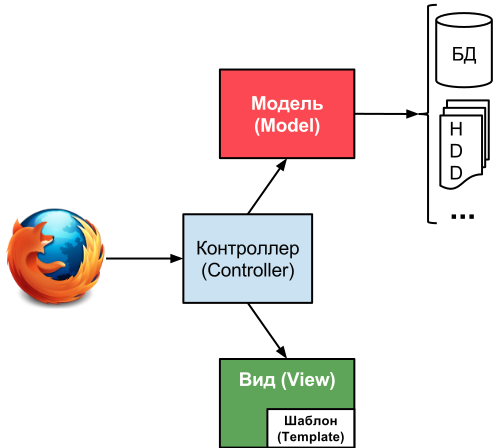
\includegraphics[width=3.2in]{media/mvc.png}
  \end{center}

\end{frame}


% Slide #9
\begin{frame}{Разделение кода: \textbf{MVC}}

  Классические \textbf{MVC} фреймворки:

  \begin{itemize}
    \item Ruby on Rails
    \item Pylons
  \end{itemize}

\end{frame}


% Slide #8
\begin{frame}{Разделение кода: \textbf{MTV}}

  Фреймворк \textbf{Django} ввел новую терминологию \textbf{MTV}

  \begin{itemize}
    \item \textbf{M -> M} Модели остались неизменными
    \item \textbf{V -> T} Представление назвали Templates
    \item \textbf{C -> V} Контроллеры назвали Views
  \end{itemize}

\end{frame}


% Slide #8
\begin{frame}{Разделение кода: \textbf{MTV}}

  Tada! Django MTV

  \begin{center}
    
\includegraphics[width=2.2in]{media/mtv_logo.jpg}
  \end{center}

\end{frame}

% Slide #8
\begin{frame}{Разделение кода: \textbf{MTV}}

  \begin{center}
    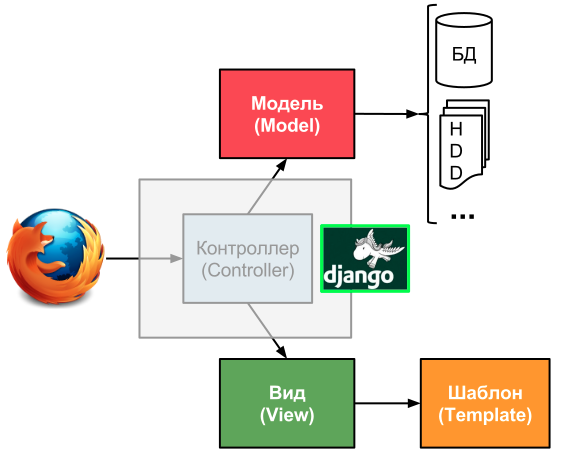
\includegraphics[width=3.2in]{media/mtv.png}
  \end{center}

\end{frame}

% Slide #11
\begin{frame}{Разделение кода: \textbf{MVC}, \textbf{MTV}, \textbf{RV}}

  Разработка без фреймворков дает вам возможность придерживаться любой
  архитектуры приложения и паттерна проектирования.

\end{frame}

% Slide #12
\begin{frame}{Разделение кода: \textbf{MVC}, \textbf{MTV}, \textbf{RV}}

  Это дает неоспоримую гибкость таким приложениям, оставляя ответственность по
  структуре ПО за разработчиком.

\end{frame}


% Slide #10
\begin{frame}{Разделение кода: \textbf{RV}}

  \textbf{RV} (Resources-View) --

  дает ту же гибкость, накладывая минимальную архитектуру идеально
  вписывающуюся в ограничения Веб приложений.

\end{frame}


% Slide #8
\begin{frame}{Разделение кода: \textbf{RV}}

  \begin{center}
    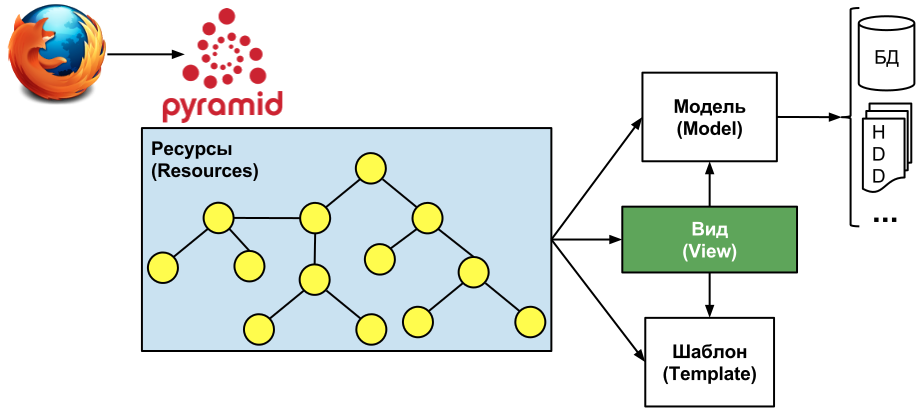
\includegraphics[width=4.0in]{media/rv.png}
  \end{center}

\end{frame}


% Slide #10
\begin{frame}{Разделение кода: \textbf{RV}}

  \say{Мы считаем, что есть только две вещи: ресурсы (\textbf{Resource}) и
    виды (\textbf{View}). Дерево ресурсов представляет структуру сайта, а вид
    представляет ресурс.
  }

\end{frame}

% Slide #10
\begin{frame}{Разделение кода: \textbf{RV}}

  \say{«\textbf{Шаблоны}» (\textbf{Template}) в реальности лишь
    деталь реализации некоторого вида: строго говоря, они не обязательны, и вид
    может вернуть ответ (Response) и без них.
  }

\end{frame}

% Slide #10
\begin{frame}{Разделение кода: \textbf{RV}}

  \say{Нет никакого «\textbf{Контроллера}» (\textbf{controller}): его просто не
    существует. «\textbf{Модель}» (\textbf{Model}) же либо представлена деревом
    ресурсов, либо «доменной моделью» (domain model) (например, моделью
    \textbf{SQLAlchemy}), которая вообще не является частью каркаса. Нам
    кажется, что наша терминология более разумна при существующих ограничениях
    веб-технологий.
  }

\end{frame}


% Slide #10
\begin{frame}{Разделение кода: \textbf{RV}}

  \textbf{Pyramid} only

    
\includegraphics[width=0.5in]{media/pyramid.png}

\end{frame}


\end{document}
